\section{$\alpha$ and $\beta$ convention}

For systems with gain, 
\begin{equation}
\tilde{\psi} \equiv \alpha \psi _1 + \beta \psi _2
\end{equation}
where $\psi _1$ is the wave function in the passive system with a center of localization at $\frac{1}{4}$L for the orientation where the wave exponentially grows to a peak before exponentially decaying to x/L=1 (left-to-right).

This then implies that $\psi _2$ is the wave function for a center of localization at $\frac{1}{4}$L for the orientation where the wave exponentially decays before growing to a peak and then decaying again (right-to-left).

\begin{figure}
\vskip -0.5cm
\centerline{
\scalebox{0.3}{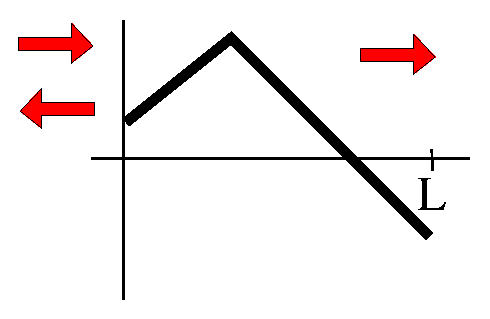
\includegraphics{pictures/transmission_derivation_14_LR}}
\scalebox{0.3}{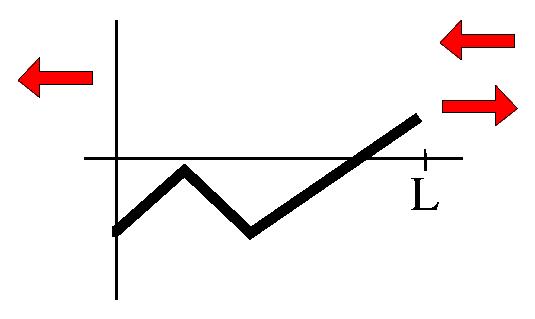
\includegraphics{pictures/transmission_derivation_34_RL}}}
\vskip -0.5cm
\caption{$\psi _1$ on the left and $\psi _2$ on the right for the passive models.}
\label{fig:alphabetacononicaldefectpositions}
\end{figure}

Similarily for $\tilde{ \psi} _1$ denoting the $\frac{1}{4}$L center of localization for left-to-right orientation and $\tilde{ \psi} _2$ being the $\frac{3}{4}$L center of localization for the right-to-left orientation.